
\documentclass{book}
\usepackage[utf8]{inputenc}
\usepackage{subcaption}
\usepackage{graphicx}
\usepackage[toc]{glossaries}
\newglossary[tlg]{technical}{tld}{tdn}{Techinical Terms}
\makeglossaries
\usepackage{hyperref}
\hypersetup{
    colorlinks,
    citecolor=black,
    filecolor=black,
    linkcolor=black,
    urlcolor=black
}

 
\title{Jaseci and Jac}
\author{Jason Mars}

\begin{document}

% \chapter*{Copyright}
% \chapter*{Acknowledgments}
% \addcontentsline{toc}{chapter}{Acknowledgments}
% \chapter*{How To Send Feedback}

\cleardoublepage % Make toc appear on right side.
\setcounter{secnumdepth}{3} % toc is 2 level deep.
\tableofcontents
\pagebreak
\printglossary[title=Terms Used, toctitle=List of Terms]
\printglossary[type=technical, title=Technical Terms Used, toctitle=List of Technical Terms]


\chapter*{Preface}
\addcontentsline{toc}{chapter}{Preface}

The way we design and write software to do computation and AI today sucks. It's a vat of boiling poop, mixed with pee, slowly swirling and bubbling toward that dehydrated semi-solid state of goop that serves to repel and repulse most normal people only attracting the few unfortunate-fortunate folks that happen to be obsessed with \gls{scat}.
\paragraph{}
Hrm, too much? Probably. I guess you'd expect me to use concrete examples and cite evidence to make my points, me being a professor and all. I mean, I could write something like \textit{``The fundamental imperative programming model utilized in near all of the production software produced in the last four decades has not changed since blah blah blah..."} to meet expections. I'd certainly sound more credible and perhaps super smart. Well, I'm not going to do that here. Let's have fun. Afterall, Jaseci has never been work for me, its play. Very ambitious play granted, but play at it's core.
\paragraph{}
Everything here is based on my opinion and intution. That suffices for me, and I hope it does for you. I have spent many decades coding and leading teams who code, but its my gut that tells me that we can do better. This book describes my attempt at better. I hope you find value in it. If you do, awesome! If you don't, also awesome.


\chapter{Introduction}


\chapter{What and Why is Jaseci?}
\section{Viewing the Problem Landscape Spacially}
\section{Compute via The Collective, The Worker Bee Model}

\chapter{Abstrations of Jaseci}
\section{Graphs}
There's something quite strange that has happend with our \gls{common languages} over the years, ...decades. When you look at it, almost every data structure we programmers use to solve problems can be modeled formally as a graph, or a special case of a graph, (save perhaps hash tables). However no common language ustilizes the formal semantics of a graph as its first order abstraction for data or memory. I mean think about it, isn't it a bit odd that practically every data structure covered in the language-agnostic classic foundational work \textit{Introduction to Algorithms}~\cite{intro_to_algo} can most naturally be be reasoned about as a graph, yet none of the common languages have built in and be designed around this primitive. I submit that the graph semantic is stupidly rich, very nice for us humans to reason about, and, most importantly for the purpose of Jaseci, is inherently well suited for a spacial conceptualization and reasoning about computational problems.
\paragraph{}
There are a few arguments that may pop into one's mind at this point of my conjecture.
\begin{itemize}
    \item ``Well there are graph libraries in my favorite language that implement graph symantics, why would I need a language to force the concept upon me?''
          or
    \item ``Duh! Interacting wi th all data and memory through graphical abstractions will make the language slow as hell since memory in hardware is essitially a big array, what is this dude talking about!?!?''
\end{itemize}
\paragraph{}
For the former question, I counter with two points. First, the core design of a language will be based upon its inherent abstractions, and with graphs not being one such abstraction the language design isn't optimized to empower programmers to nimbly do fancy gymnastics with the rich symantics of graphs. And second, libraries suck (See~\ref{rant:librariessuck}).
\paragraph{}
For the latter question, I'd respond, ``Have you SEEN the kind of abstractions in modern languages!?!? It's rediculous, lets look at python dictionaries, actually scratch that, lets keep it simple and look at dynamic typing in general. The runtime complexity to support dynamic typing is most certainly hgiher than a graph abstraction. Duh right back at'ya!''
\subsection{Yes, But What Kind of Graphs}
\begin{figure}
    \begin{subfigure}{.5\textwidth}
        \centering
        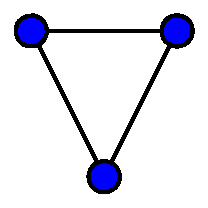
\includegraphics[width=.8\linewidth]{assets/images/Undirected.svg.pdf}
        \caption{1a}
        \label{fig:sfig1}
    \end{subfigure}%
    \begin{subfigure}{.5\textwidth}
        \centering
        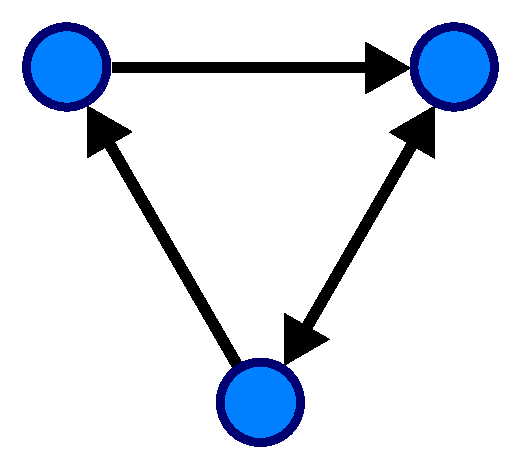
\includegraphics[width=.8\linewidth]{assets/images/Directed.svg.pdf}
        \caption{1b}
        \label{fig:sfig2}
    \end{subfigure}
    \begin{subfigure}{.5\textwidth}
        \centering
        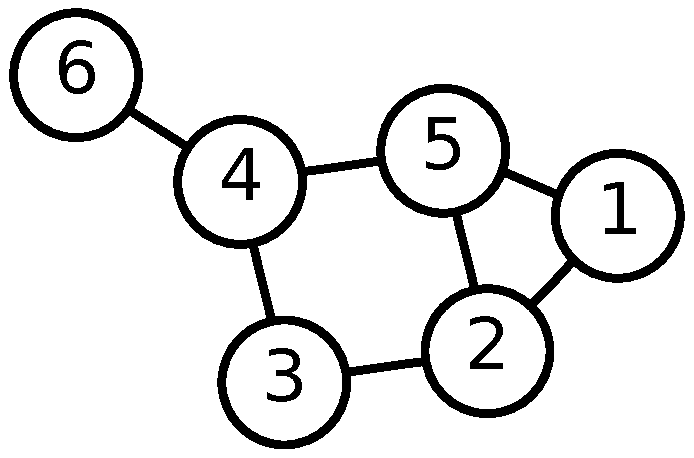
\includegraphics[width=.8\linewidth]{assets/images/6n-graf.svg.pdf}
        \caption{1a}
        \label{fig:sfig1}
    \end{subfigure}%
    \begin{subfigure}{.5\textwidth}
        \centering
        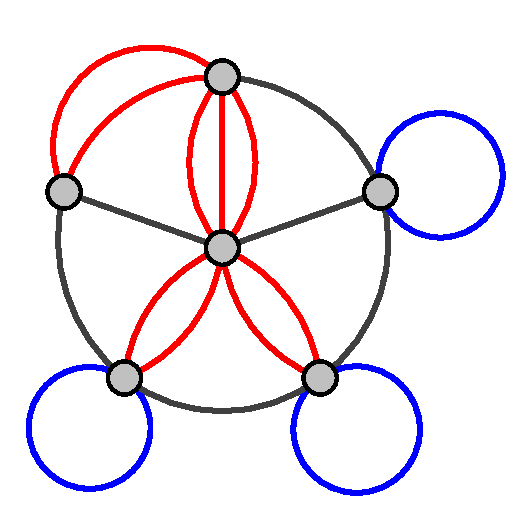
\includegraphics[width=.8\linewidth]{assets/images/Multi-pseudograph.svg.pdf}
        \caption{1b}
        \label{fig:sfig2}
    \end{subfigure}
    \begin{subfigure}{.5\textwidth}
        \centering
        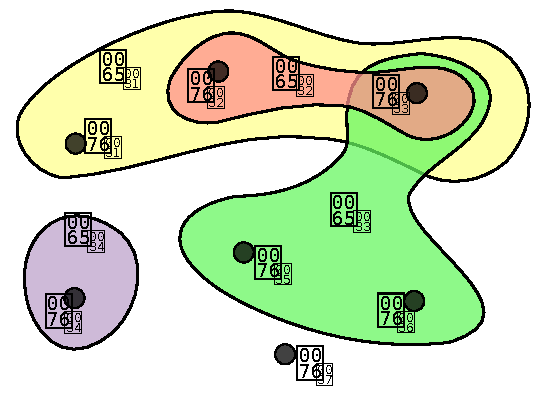
\includegraphics[width=.8\linewidth]{assets/images/Hypergraph-wikipedia.svg.pdf}
        \caption{1a}
        \label{fig:sfig1}
    \end{subfigure}%
    \begin{subfigure}{.5\textwidth}
        \centering
        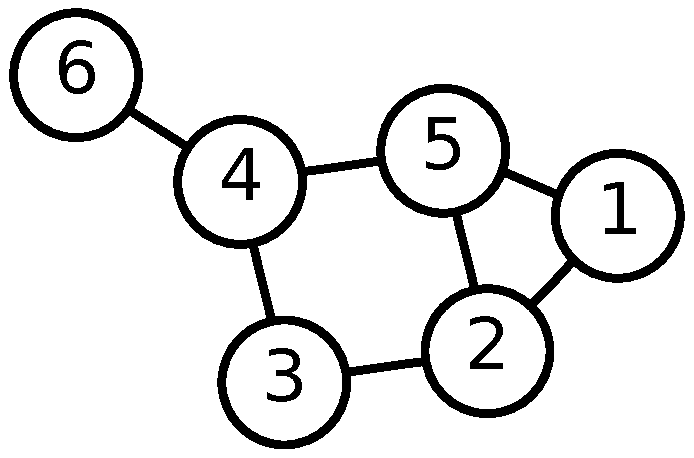
\includegraphics[width=.8\linewidth]{assets/images/6n-graf.svg.pdf}
        \caption{1b}
        \label{fig:sfig2}
    \end{subfigure}
    \caption{plots of....}
    \label{fig:fig}
\end{figure}
There are many categories of graphs to consider when thinking about the abstraction to add to Jaseci. There are \gls{directed graphs}, \gls{undirected graphs}, \gls{multigraphs}, non-multigraphs, \gls{hypergraphs}, and any combination of the lot.
\subsection{Nodes}
\subsection{Edges}

\section{Walkers}
\section{Abilities}
\section{Other Abstractions Not Yet Actualized}

\chapter{Architecture of Jaseci and Jac}
\section{Anatomy of a Jaseci Application}
\section{The Jaseci Machine}
\subsection{Machine Core}
\subsection{Jaseci Cloud Server}

\chapter{Interfacing a Jaseci Machine}
\section{JSCTL: The Jaseci Command Line Interface}
\section{Jaseci Rest API}

\chapter{The Jac Programming Language}


\chapter{Architecting Jaseci Core}

\chapter{Architecting Jaseci Cloud Serving}

\chapter*{Epilogue}
\addcontentsline{toc}{chapter}{Epilogue}

\appendix
\chapter{Rants}
\section{Why Libraries Suck}
\label{rant:librariessuck}
\paragraph{}
Because they do.
\paragraph{}
Still need more reasons?
\paragraph{}
Well, if you dont already know, I'm not going to tell you.
\paragraph{}
Fine, I'll tell you.
\begin{enumerate}
    \item They suck because they create dependancies for which you must have faith in the implementer of the library to maintain and keep bug free.
    \item They suck because there are often at least 10 options to choose from with near exact features expressings slightly different idosyncratic ways.
    \item They suck because they suck.
\end{enumerate}
Don't get me wrong, we have to use libraries. I'm not saying go reimplement the wheel 15 thousand times over. But that doesn't mean they don't suck and should be avoided if possible. The best is to know your library inside and out so the moment you hit some suckitude you can pull in the library's source code into your own codebase and \gls{pwn} it as your own.

\newglossaryentry{christen}
{
    name=christen,
    description={to name or dedicate (something, such as a piece of code) by a ceremony that often involves breaking a bottle of champagne}
}
\newglossaryentry{scat}
{
    name=scat,
    description={the excrement of an animal including but not limited to human; also heroin }
}
\newglossaryentry{pwn}
{
    name=pwn,
    description={the act of dominating a person, place, or thing. (...or a piece of code)}
}
\newglossaryentry{gobbledygook}
{
    name=gobbledygook,
    description={language that is meaningless or is made unintelligible by excessive use of abstruse technical terms; nonsense}
}
\newglossaryentry{bleh}
{
    name=bleh,
    description={mildly yucky}
}
\newglossaryentry{leet}
{
    name=leet,
    description={v. hyper-sophisticated from a coding perspective, n. a language used by \gls{leet} \gls{haxor}s}
}

\newglossaryentry{haxor}
{
    name=haxor,
    description={\gls{leet} spelling of hacker}
}
\newglossaryentry{coder}
{
    name=coder,
    description={the superior human}
}
\newglossaryentry{Jaseci jolt}
{
    name=Jaseci jolt,
    description={an insight derived from Jaseci that serves as a high voltage bolt of energy to the mind of a sharp coder.}
}
\newglossaryentry{common languages}
{
    name=common languages,
    description={typical languages programmers use to write commercial software, (e.g., C, C++, Java, Javascript, Python, Ruby, Go, Perl, PHP, etc.)}
}

\newglossaryentry{grok}
{
    name=grok,
    description={to fully comprehend and understand deeply }
}

\newglossaryentry{sick}
{
    name=sick,
    description={\gls{redonkulous}}
}

\newglossaryentry{redonkulous}
{
    name=redonkulous,
    description={\gls{dope}}
}

\newglossaryentry{dope}
{
    name=dope,
    description={\gls{sick}}
}

\newglossaryentry{goo goo gaa gaa}
{
    name=goo goo gaa gaa,
    description={the language of babies}
}

\newglossaryentry{directed graphs}
{
    type=technical,
    name=directed graphs,
    description={}
}
\newglossaryentry{undirected graphs}
{
    type=technical,
    name=undirected graphs,
    description={}
}

\newglossaryentry{multigraphs}
{
    type=technical,
    name=multigraph,
    description={}
}

\newglossaryentry{hypergraphs}
{
    type=technical,
    name=hypergraph,
    description={}
}

\newglossaryentry{contexts}
{
    type=technical,
    name=contexts,
    description={A set of key value pairings that serve as a data payload attributable to nodes and edges in Jaseci graphs}
}

\newglossaryentry{walker}
{
    type=technical,
    name=walker,
    description={An abstraction in the Jaseci machine and Jac programming language that represents a computational agent that computes and travels along nodes and edges of a graph}
}


\bibliographystyle{plain}
\bibliography{book}
\end{document}
